%%%%%%%%%%%%%%%%%%%%%%%%%%%%%%%%%%%%%%%%%%%%%%%%%%%%%%%%%%%%%%%
%
% Welcome to Overleaf --- just edit your LaTeX on the left,
% and we'll compile it for you on the right. If you open the
% 'Share' menu, you can invite other users to edit at the same
% time. See www.overleaf.com/learn for more info. Enjoy!
%
%%%%%%%%%%%%%%%%%%%%%%%%%%%%%%%%%%%%%%%%%%%%%%%%%%%%%%%%%%%%%%%


% Inbuilt themes in beamer
\documentclass{beamer}

\usepackage{booktabs}
% Theme choice:
\usetheme{CambridgeUS}

% Title page details: 
\title{ASSIGNMENT 4} 
\author{CS21BTECH11020}
\date{\today}
\logo{\large \LaTeX{}}


\begin{document}

% Title page frame
\begin{frame}
    \titlepage 
\end{frame}

% Remove logo from the next slides
\logo{}


% Outline frame
\begin{frame}{Outline}
    \tableofcontents
\end{frame}


% Lists frame
\section{Problem Statment}

\begin{frame}{Problem Statment}
    \begin{block}{Class 11 Probability Ex 16.3 Q19}
        In an entrance test that is graded on the basis of two examinations,the probability of randomly chosen studnet passing the first examination is 0.8 and the probability of passing the second examination is 0.7. The probability of passing atleast one of them is 0.95. What is the probability of passing both ?    
    \end{block}
\end{frame}

\section{Solution}

\begin{frame}{Solution}
    There are two exams: Exam A and Exam B \\
    Let Random varaibles X and Y represent Status of Exam A and Exam B respectively.\\
    \begin{table}
        \begin{tabular}{|c|c|c|}
            \hline
            & Fail & Pass \\
            \hline
            X & 0 & 1 \\
            \hline
            Y & 0 & 1 \\
            \hline
        \end{tabular}
    \end{table}
    \begin{block}{Given Data}
        \begin{align}
            P_X(X = 1) &= 0.8 \label{eq:1}\\
            P_Y(Y = 1) &= 0.7 \label{eq:2}\\
            P_{X+Y}(X+Y = 1) &= 0.95 \label{eq:3}
        \end{align}
    \end{block}
\end{frame}


\begin{frame}{Continued ...}
        \begin{alertblock}{Principle of Inclusion And Exclusion}
           It states that for finite sets $ A_1,...,A_n$, one has the identity\\
           \begin{equation}
               \left| \bigcup_{i=1}^n A_i \right| = \sum_{\phi J \subseteq \{1,\ldots,n \}} (-1)^{|J|+1} \left| \bigcap_{j \in J} A_j \right| \label{eq:4}
           \end{equation}
        \end{alertblock}
        \begin{block}{}
            Using equation \eqref{eq:4}, we have \\
            \begin{equation}
                P_{X+Y}(X+Y) = P_X(X) + P_Y(Y) - P_{XY}(XY)
            \end{equation}
            Using \eqref{eq:1},\eqref{eq:2} and \eqref{eq:3}, we get
            \begin{align}
                0.95 &= 0.8 + 0.7 -P_{XY}(XY = 1) \\
                P_{XY}(XY = 1) &= 0.55
            \end{align}

        \end{block}
        
\end{frame}

\section{Python Code}
\begin{frame}{Python Code}
    

\begin{figure}
    \centering
    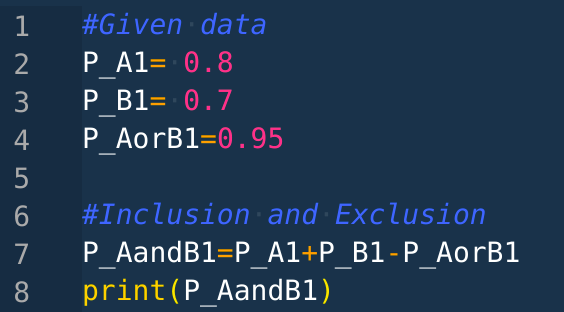
\includegraphics[scale = 0.4]{./python.png}
\end{figure}
\end{frame}



\end{document}